\documentclass[xcolor=dvipsnames]{beamer}
\usepackage{listings}
\usepackage[T1]{fontenc}
\usepackage{lmodern}
\usepackage[utf8]{inputenc}
\usepackage{textpos}
\usepackage{color}
\usepackage{hyperref}

% \usepackage[swedish]{babel} %To get a swedish style of the document, swedish typographical rules and so on

\lstset{language=D}          % Set your language (you can change the language for each code-block optionally)
\lstset{basicstyle=\footnotesize\ttfamily,breaklines=true}
\lstset{language=D,
  basicstyle=\ttfamily\scriptsize,
  keywordstyle=\color{blue}\ttfamily,
  stringstyle=\color{red}\ttfamily,
  commentstyle=\color{brown}\ttfamily,
  morecomment=[l][\color{magenta}]{\#}
}

\usetheme{Boadilla}              %default, Boadilla
\usecolortheme[named=Maroon]{structure}

\title[Error Handling \& D]{Error Handling \& D}
\author[Per Nordlöw% , HiQ
]{\textbf {Per Nordlöw% \\HiQ
  }} % auteur

% \useoutertheme{umbcfootline}
\setbeamertemplate{background canvas}[vertical shading][bottom=red!20,top=yellow!30]
% \setbeamertemplate{background}[grid][step=5mm,color=blue]
% \setbeamertemplate{background}{\includegraphics[width=\paperwidth]{sunset.jpg}}

\begin{document}

% Titleframe
\begin{frame}[fragile]
  \begin{figure}
    \fbox{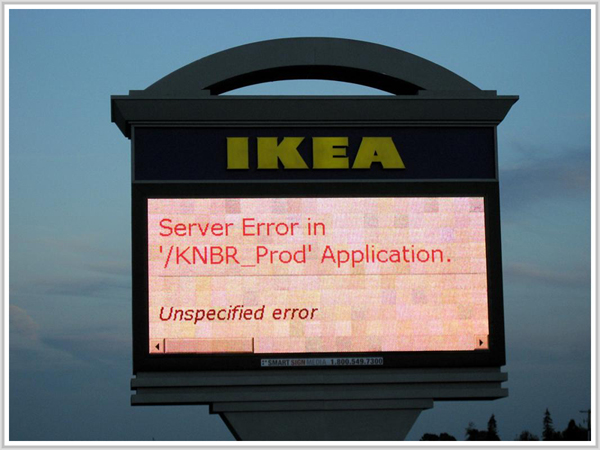
\includegraphics[width=0.6\textwidth]{ikea}}
  \end{figure}
  \maketitle
\end{frame}

% \addtobeamertemplate{frametitle}{}{%
% \begin{textblock*}{100mm} (.85\textwidth,-0.5cm)
% 
\includegraphics[height=1cm,width=2cm]{hiq}
% \end{textblock*}}

\begin{frame}[fragile]{Machines, Software and Trust}
  \begin{figure}
    \fbox{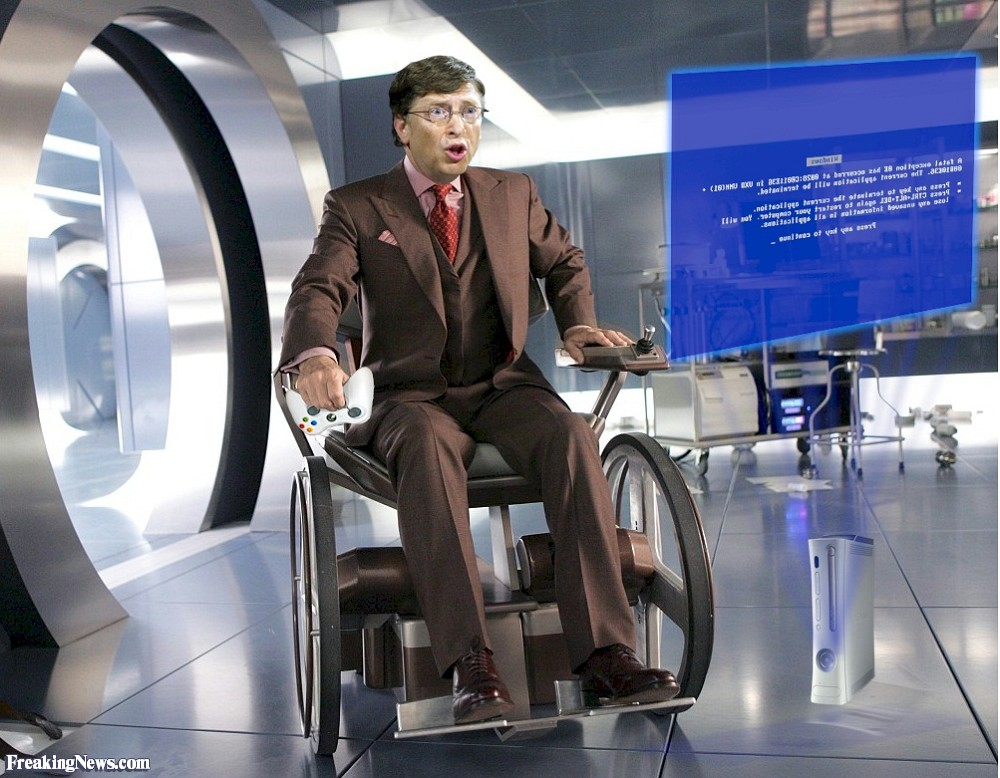
\includegraphics[width=0.5\textwidth]{xman}}
  \end{figure}
  \begin{itemize}[<+->]
  \item Why do \textit{todays} programs crash?
  \item Car Bulb Analogy
  \item \emph{Must} they?
  \item How to fix it
  \item D is one step forward\ldots
  \end{itemize}
\end{frame}

\begin{frame}[fragile]{Trend: It's human to err!}
  \begin{figure}
    \fbox{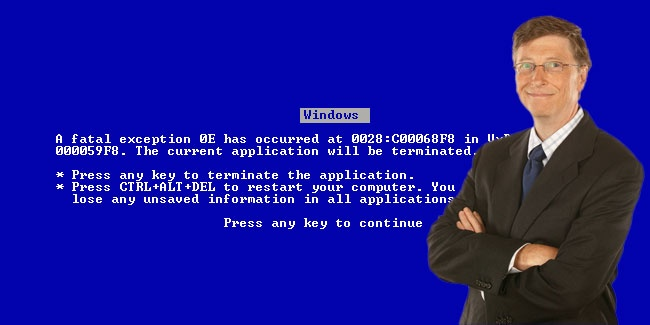
\includegraphics[width=0.72\textwidth]{human2err}}
  \end{figure}
  \begin{itemize}[<+->]
  \item Legacy: Humans don't err
  \item Changing Tides
    \begin{itemize}[<+->]
    \item Git: Mistakes Allowed: ``Rewrite history''
    \item No Programming Priesthood
    \end{itemize}
  \item Humans \& Machine Redundance
  \item Error Correction
  \item Error Resilience
  \end{itemize}
\end{frame}

\begin{frame}[fragile]{Software Process Goal:\\Detect Errors as \emph{Early as} Possible}
  % \fbox{\centering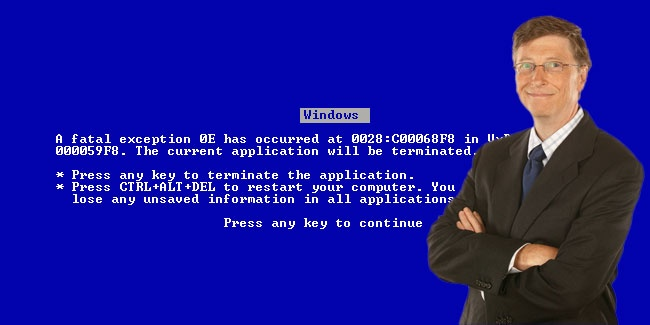
\includegraphics[width=0.8\textwidth]{human2err}}
  \begin{itemize}[<+->]
  \item \textbf{Build} (Compile, Link): Static Syntax \& Semantic Checking
  \item \textbf{Test}: Dynamic Checking
  \item \textbf{Run}: Dynamic Checking
  \end{itemize}
\end{frame}

\begin{frame}[fragile]{Type System is the Key}
  \begin{itemize}[<+->]
  \item Information Propagation (DRY): Reflection
  \item Rich Type Programming: Default, Range, Step, Saturation, Physical Unit
  \item Requires \emph{Formal} Language to Capture its Algebra!
  \item Type Inference: Unit Analysis
  \item \emph{Type Safe Linking}: Should Change Everything! We just need to
    fixed GNU ld. GCC already puts types in debug information.
  \item Trend: Static code inference can give guarantees on
    (concurrent) code!:\\
    Examples: Rust, Haskell, D, Scala, OCaml, F\#, Julia partly C\#
  \end{itemize}
\end{frame}

\begin{frame}[fragile]{Error Handling Alternatives}
  \begin{itemize}[<+->]
  \item \textbf{Return Value}:
    \begin{itemize}[<+->]
    \item Nobody checks return of \texttt{printf} nor \texttt{malloc} in C.
    \item Try running programs on a system almost out of memory or disk.
    \end{itemize}
  \item \textbf{Exceptions}:
    \begin{itemize}[<+->]
    \item Stroustrup on its performance
    \item Almost religious wars
    \item Polynomial Complexity
    \item Cleanup scope
    \item Exception safe constructors
    \end{itemize}
  \item \textbf{Scope}:
    \begin{itemize}[<+->]
    \item D-only
    \item Linear complexity
    \item Compiler generates nested try-catch expressions.
    \end{itemize}
  \end{itemize}
\end{frame}

\begin{frame}[fragile]{Redundancy}
  \begin{figure}
    \fbox{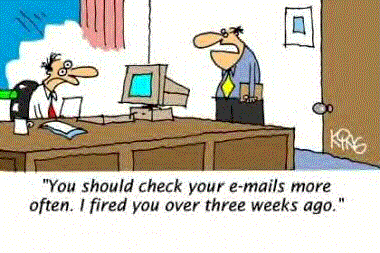
\includegraphics[width=0.50\textwidth]{fired}}
  \end{figure}
  % \begin{figure}
  %   \fbox{
\includegraphics[width=0.50\textwidth]{cat}}
  % \end{figure}
  \begin{itemize}[<+->]
  \item Compactest code is random but impossible to understand and correct
  \item Managers!: Computers have no common sense!
  \item Not just numerics but
  \item Units, Default-Value, Range, Saturation, Ownership, Access, etc
  \end{itemize}
\end{frame}

\begin{frame}[fragile]{Interaction with Structured Information}
  \begin{itemize}[<+->]
  \item Limit input to very specific structure in
  \item GUI/Webb Forms
  \item Example: Personal Codes, Dates, etc
  \item Lazy Programmers: Integrate pattern matching with UI component input
    logic and reuse!
  \item Leaders!: Investment always pays off in the long run!
  \end{itemize}
\end{frame}

\begin{frame}[fragile]{General Tips}
  \begin{itemize}[<+->]
  \item Minimize Number of \textbf{Configurations}, especially in dynamic languages
  \item Minimize Number of \textbf{Code Paths}
  \item Learn \& Use \textbf{Reflection} (Static \& Dynamic) =>
  \item \textbf{Propagate Information Structure} to
    \begin{itemize}[<+->]
    \item Command Line
    \item GUIs
    \item Protocols (showcase Boost.Serialization)
    \item etc
    \end{itemize}
  \item Make it impossible for user to enter incorrectly formatted data
  \item Separate logic from presentation (CSS, LaTeX, Qt-XML)
  \end{itemize}
\end{frame}

\begin{frame}[fragile]{Dinner!}
  \begin{figure}
    \fbox{
\includegraphics[width=1.0\textwidth]{werewolf}}
  \end{figure}
\end{frame}

\begin{frame}[fragile]{Iron Man like Systems and Interfaces?}
  How do we turn software engineers into Tony Starks? :)
  \begin{figure}
    \fbox{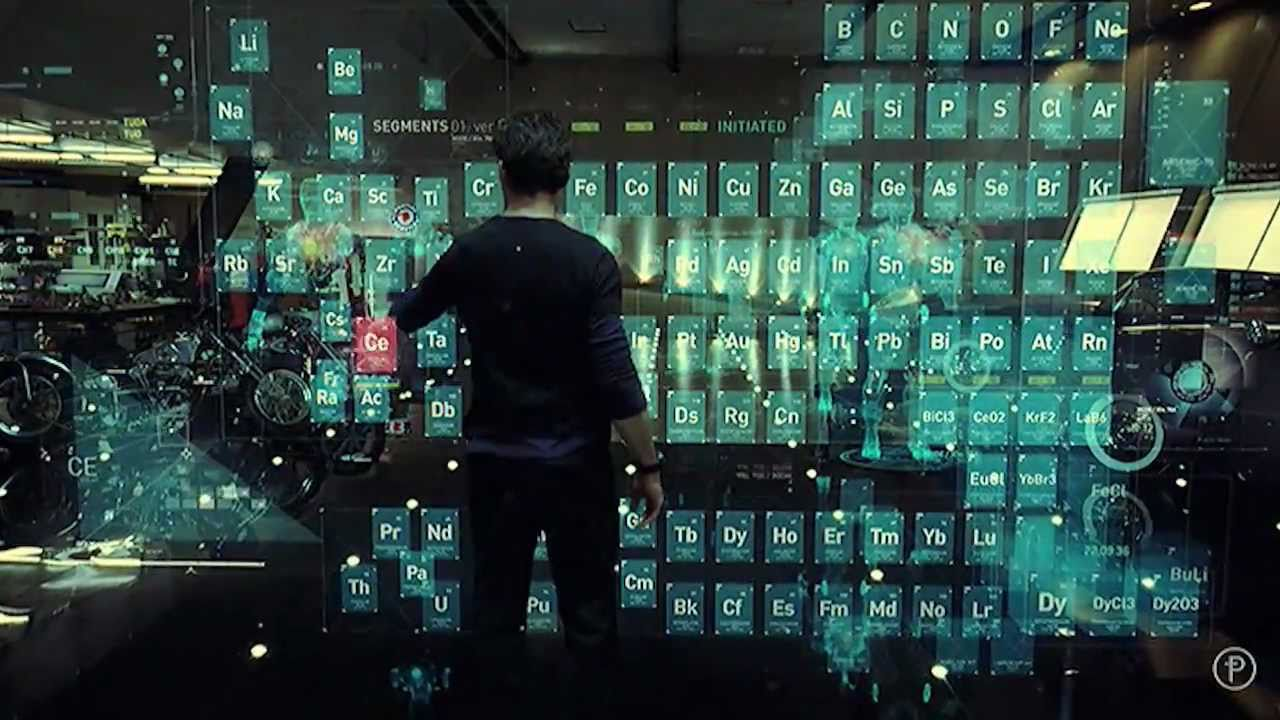
\includegraphics[width=0.60\textwidth]{stark}}
  \end{figure}
  and what language shall we bootstrap this with!? We need it to be
  \begin{itemize}[<+->]
  \item \textbf{Safe}: Provably Correct Memory Accesses
  \item \textbf{Performant}: (Fast Build and Run of Native Code)
  \item \textbf{Effective}: Easy, Expressive, Creative, Joyful
  \end{itemize}

  \begin{itemize}[<+->]
  \item \textbf{Other}: Only 2 out of 3
  \item \textbf{D}: 3 out 3!
  \end{itemize}
\end{frame}

\begin{frame}[fragile]{Leading Questions}
  \begin{itemize}[<+->]
  \item Why do systems \emph{keep on} crashing?
  \item Why do projects need so many languages: SAAB SimC uses C/C++, Fortran,
    Ada, Python, Shell, Make, \ldots =>
  \item Restrictive languages, such as Ada, looses all its safety in the
    wrapping layer.
  \item Background for Ada: Before 100s of langs in US Defence
  \item Why do we keep on torturing ourselves with obselete/faulty languages?
  \item Why am I doing this?
    \begin{itemize}[<+->]
    \item About me
    \item Time
    \item Age
    \item Lifes too short for bad code
    \end{itemize}
  \item Either stick with it, or try to change it:
  \item Help/Promote D and alikes
  \item Get to work with what I find meaningful
  \end{itemize}
\end{frame}

\begin{frame}[fragile]{Language Trend}
  \begin{itemize}[<+->]
  \item Statically Inferred Languages
  \item Game Industry: ``Good C++ programmers are hard to find''. Why?
  \item Mozilla: Servo Layout Engine using Rust
  \item Microsoft Announcement: ``We are planning a new language that is''
    \begin{itemize}[<+->]
    \item ``as fast as C++'' and
    \item ``as simple as C\#''
    \end{itemize}
  \item D already does this in company production code
  \end{itemize}
\end{frame}

\begin{frame}[fragile]{Why should you learn about D?}
  Not Just Compacter Syntax but
  \begin{itemize}[<+->]
  \item \textbf{Proving Ground} for Future C++
  \item \textbf{Just like Market Consumers}:
  \item \textbf{Developer have Responsibility}:
    \begin{itemize}[<+->]
    \item If we aren't aware
    \item We won't ask for it and
    \item We will not get it (in languages in general)
    \end{itemize}
  \end{itemize}
\end{frame}

\begin{frame}[fragile]{Democratic \& Pragmatic Fundaments}
    \begin{columns}[c] % the "c" option specifies center vertical alignment
      \column{.65\textwidth}
      \begin{itemize}[<+->]
      \item Gold is \emph{not} everything that\ldots --- Big leaps are
        \emph{not} made by large companies nor organisations.
      \item \textbf{Dynamic}: Non-Company Controlled: no more: \textit{``Lets reinvent
          everything again just because we want to be different!''}
      \item \textbf{No Priesthood} nor too Academic
      \item We have done our homework!
      \item C/C++/C\#-like to \textbf{ease transition}
      \item \textbf{Pragmatic}: Developers want to GTD
      \item \textbf{Democratic/Dynamic}: Key solutions voted for. All about
        \emph{probabilities}.
      \item \textbf{Continuous Integration} on Github
      \end{itemize}
      \column{.35\textwidth}
      \begin{figure}
        \fbox{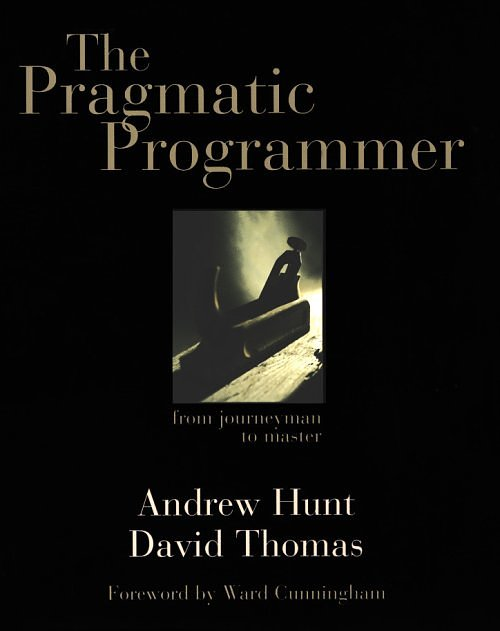
\includegraphics[width=0.9\textwidth]{pragmatic}}
      \end{figure}
    \end{columns}
\end{frame}

\begin{frame}[fragile]{The Scientist and The Craftman --- D's Magic Pair!}
  \begin{figure}
    \fbox{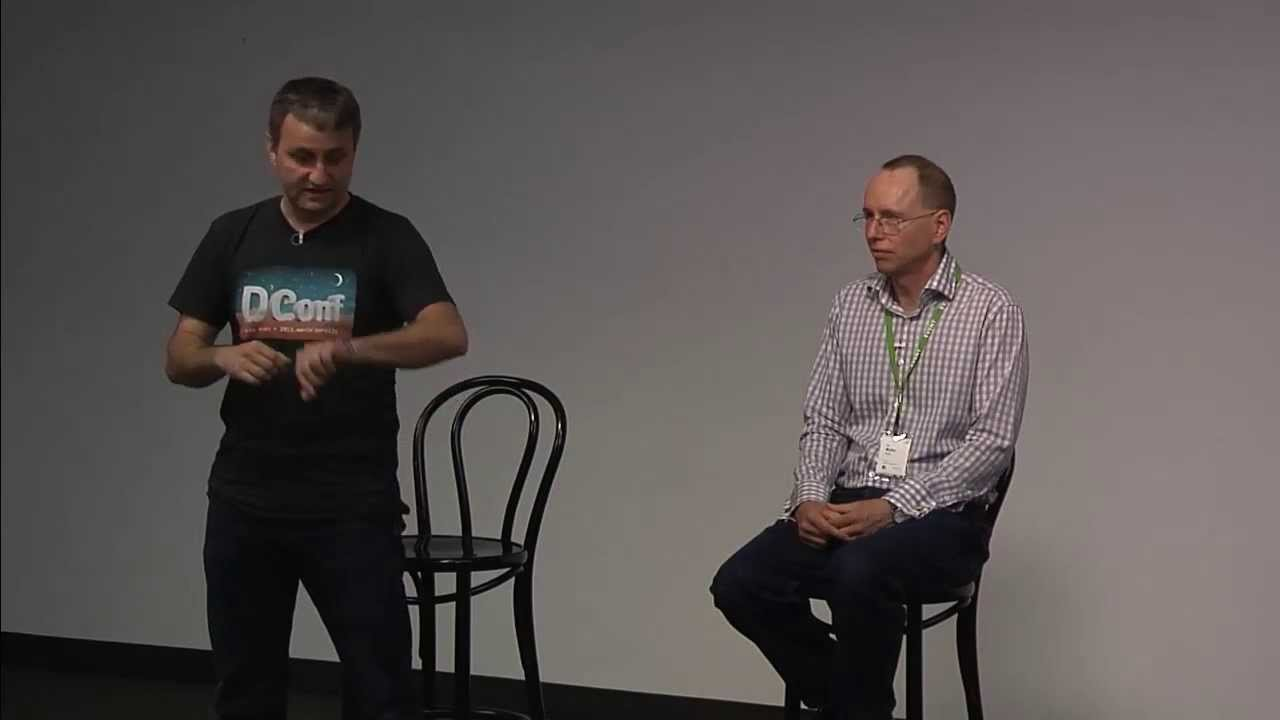
\includegraphics[width=0.80\textwidth]{andreibright}}
  \end{figure}
 \pause{}
  \begin{itemize}[<+->]
  \item History and Development of Walter Bright and D is very similar to that
    of Linus Torvalds and Linux.
  \end{itemize}
\end{frame}

\begin{frame}[fragile]{Heart of D: Reuseable Software}
  \begin{figure}
    \fbox{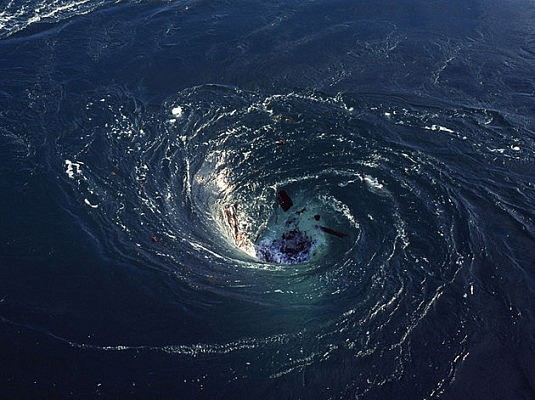
\includegraphics[width=0.6\textwidth]{whirl}}
  \end{figure}
 Walter Bright: How can we
 \pause{}
  \begin{itemize}[<+->]
  \item Write truly reusable software components?
  \item Escape ``Whirlpool Programming''?
  \end{itemize}
\end{frame}

\begin{frame}[fragile]{Heart of D: Component Programming Pipeline}
  \begin{figure}
    \fbox{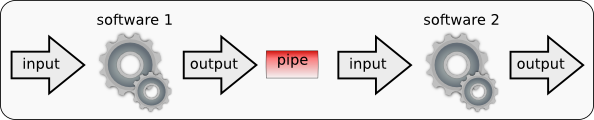
\includegraphics[width=1.0\textwidth]{pipe}}
  \end{figure}
  Successful model in
  \begin{itemize}[<+->]
  \item As Western text: Left-to-right
  \item Proof of Concept: UNIX Commands \& Pipes
  \end{itemize}
\end{frame}

\begin{frame}[fragile]{Heart of D: Component Programming Example}
  ``Read lines, sort em and print em back'':
\begin{lstlisting}[frame=single]
import std.stdio, std.algorithm, std.range, std.array;
void main(string args[]) {
    Stdin.
        byLine(KeepTerminator.yes).
        map!(a => a.idup).
        array.
        sort.
        copy(stdout.lockingTextWriter());
}
\end{lstlisting}
as fast as handwritten C with nested loops and with manual error-checking but
way simpler and more flexible
\end{frame}

\begin{frame}[fragile]{Heart of D: Component Programming realized by}
  \begin{itemize}[<+->]
  \item \textbf{Generics} (= reuse) made simple
  \item \textbf{Ranges}
    \begin{itemize}[<+->]
    \item Lazy/Delayed Evaluated means
    \item Return Calculation instead of Value
    \item Also called Higher-Order Range Pattern
    \item Compare with Monad
    \item Example:
      \begin{lstlisting}[frame=single]
        writeln(x,y,z); // no allocation
        writeln(x~y~z); // heap allocates
      \end{lstlisting}
    \item Concept easily confused with \emph{value} ranges such as Ada's
      \emph{Range Types}
    \end{itemize}
  \item \textbf{Arrays} and \textbf{Strings} Done Right
  \item Uniform Call Syntax (\textbf{UFCS})
  \item Compile-Time Function Evaluation (\textbf{CTFE})
  \item \textbf{Emptyness Propagation}: no if statments to check for null etc
    enables. Removes Error handling problem!
  \item \textbf{Concepts}: (Type Predicates)
  \item \textbf{Inlining} instead of function calls
  \end{itemize}
\end{frame}

\begin{frame}[fragile]{Uniform Call Syntax (UFCS)}
  \begin{itemize}[<+->]
  \item to! makes API-integration transparent
  \item \texttt{needle.findIn(haystack)} is more obvious than
  \item \texttt{findIn(needle, haystack)} and is used in
  \item module \texttt{msgpack-d} as
    \begin{itemize}[<+->]
    \item \texttt{value.pack}
    \item \texttt{value.unpack}
    \end{itemize}
  \item Chained Left-to-Right: \texttt{data.doThis.doThat;}
  \item Ruby-Style: \texttt{"/bin/ls".isFile}
  \end{itemize}
\end{frame}

% %%%%%%%%%%%%%%%%%%%%%%%%%%%%%%%%

\begin{frame}[fragile]{Concepts \& Ranges}
    \begin{itemize}[<+->]
    \item AI The Movei Robotic Spare Arm Analog: Body is Range and Arm is
      Algorithm/Range
    \item Algorithms are the axioms and always come first
      \begin{itemize}[<+->]
      \item \texttt{reverse}
      \item \texttt{editDistance}
      \item \texttt{binarySearch}, \texttt{quickSort}
      \end{itemize}
    \item Concepts/Ranges (Minimal Data Interface Requirements) follow that groups
    \item Containers
    \item Example: Check if a \texttt{range} is a \textbf{Palindrome}
    \begin{lstlisting}[frame=single]
bool isPalindrome(Range)(in Range x)
if (isBidirectionalRange!Range) {
    import std.algorithm: retro, equal;
    return x.retro.equal(x);
}
    \end{lstlisting}
    \end{itemize}
\end{frame}

\begin{frame}[fragile]{Concepts \& Ranges}
  \begin{itemize}[<+->]
  \item Minimal set of requirements of interfaces to types gives
  \item Ranges and Interfaces.
  \item Example \texttt{binarySearch} and \texttt{quickSort} works on anything
    that provides \textbf{RandomAccess}.
  \item Distinguish between
    \begin{itemize}[<+->]
    \item \textbf{std.range}: return calculations (like C++ expression templates
      but way simpler)
    \item \textbf{std.algorithm}: return values
    \end{itemize}
  \item A must need in Linear Algebra Packages
  \end{itemize}
\end{frame}

\begin{frame}[fragile]{Concepts \& Ranges}
  \begin{itemize}[<+->]
  \item More Compact/Efficient Encoding (Development) of Algorithms and their
    Variants (in Phobos)
  \item Unique Feature of D: Ranges preserve powers when possible.
    \begin{lstlisting}[frame=single]
auto y = x.map("a*a")}.
    \end{lstlisting}
      If \texttt{x} is random access \texttt{y} also is
  \item \texttt{std.array}: \texttt{array} triggers computation if input is not RandomAccess
  \item See Andrei Alexandrescous article "Forward is Not Enough"
  \item Ranges and algorithms are more generic than others (STL). For example
    search/find can search for multiple (variadic) keys.
  \item TODO: Visualizations of behaviour would be nice
  \end{itemize}
\end{frame}

\begin{frame}[fragile]{List of Range Creations 1}
  \begin{itemize}[<+->]
  \item \textbf{\texttt{retro}}: Iterates a bidirectional range \emph{backwards}.
  \item \textbf{\texttt{stride}}: Iterates a range with \emph{stride} \texttt{n}.
  \item \textbf{\texttt{chain}}: \emph{Concatenates} several ranges into a single range.
  \item \textbf{\texttt{roundRobin}}: Given n ranges, creates a new range that return the
    n first elements of each range, in turn, then the second element of each
    range, and so on, in a round-robin fashion.
  \item \textbf{\texttt{radial}}: Given a random-access range and a starting point,
    creates a range that alternately returns the next left and next right
    element to the starting point.
  \item \textbf{\texttt{take}}: Creates a sub-range consisting of only up to the first n
    elements of the given range.
  \item \textbf{\texttt{takeExactly}}: Like take, but assumes the given range actually
    has n elements, and therefore also defines the length property.
  \item \textbf{\texttt{takeOne}}: Creates a random-access range consisting of exactly
    the first element of the given range.
  \item \textbf{\texttt{takeNone}}: Creates a random-access range consisting of zero elements of the given range.
  \end{itemize}
\end{frame}

\begin{frame}[fragile]{List of Range Creations 2}
  \begin{itemize}[<+->]
  \item \textbf{\texttt{drop}}: Creates the range that results from discarding the first
    n elements from the given range.
  \item \textbf{\texttt{dropExactly}}: Creates the range that results from discarding
    exactly n of the first elements from the given range.
  \item \textbf{\texttt{dropOne}}: Creates the range that results from discarding the
    first elements from the given range.
  \item \textbf{\texttt{repeat}}: Creates a range that consists of a single element
    repeated n times, or an infinite range repeating that element indefinitely.
  \item \textbf{\texttt{cycle}}: Creates an infinite range that repeats the given forward
    range indefinitely. Look ma no types!:
    \begin{lstlisting}[frame=single]
import std.range;
auto b = [1,2,3,4]; // buffer
auto cb = b.cycle; // circular buffer
    \end{lstlisting}
  \item \textbf{\texttt{zip}}: Given n ranges, creates a range that successively returns
    a tuple of all the first elements, a tuple of all the second elements, etc.
  \item \textbf{\texttt{lockstep}}: Iterates n ranges in lockstep, for use in a foreach
    loop. Similar to zip, except that lockstep is designed especially for
    foreach loops.
  \item \textbf{\texttt{recurrence}}: Creates a forward range whose values are defined by
    a mathematical recurrence relation.
  \end{itemize}
\end{frame}

\begin{frame}[fragile]{List of Range Creations 3}
  \begin{itemize}[<+->]
  \item \textbf{\texttt{sequence}}: Similar to recurrence, except that a random-access
    range is created.
  \item \textbf{\texttt{iota}}: Creates a range consisting of numbers between a starting
    point and ending point, spaced apart by a given interval.
  \item \textbf{\texttt{frontTransversal}}: Creates a range that iterates over the first
    elements of the given ranges.
  \item \textbf{\texttt{transversal}}: Creates a range that iterates over the n'th
    elements of the given random-access ranges.
  \item \textbf{\texttt{indexed}}: Creates a range that offers a view of a given range as
    though its elements were reordered according to a given range of indices.
  \item \textbf{\texttt{chunks}}: Creates a range that returns fixed-size chunks of the
    original range.
  \item \textbf{\texttt{only}}: Creates a range that iterates over a single value.
  \end{itemize}
\end{frame}

\begin{frame}[fragile]{Data Semantics}
  \begin{itemize}[<+->]
  \item Like in C\#
  \item Clear Distingushing between
    \begin{itemize}[<+->]
    \item \emph{Value} Semantics: \texttt{struct}
    \item \emph{Reference} Semantics: \texttt{class}
    \end{itemize}
  \item Removes need for C++'s pointer member access operator: \texttt{->}
  \end{itemize}
\end{frame}

\begin{frame}[fragile]{Safer and Easier Class Polymorphism}
  \begin{itemize}[<+->]
  \item \emph{All} members functions by default virtual
  \item No \texttt{virtual} keyword needed
  \item Overriding must be explicit through \texttt{override}
  \item Member qualifier \texttt{final} makes them non-virtual
  \item Final members can't be overridden in sub-classes
  \end{itemize}
\end{frame}

\begin{frame}[fragile]{Basic Needs Builtin}
  \begin{itemize}[<+->]
  \item Strings: \texttt{string}
  \item Arrays: \texttt{ubyte[]}
  \item Maps (Associative Arrays): \texttt{ubyte[string]}
  \end{itemize}
\end{frame}

\begin{frame}[fragile]{Arrays Done Right fixes ``C's Largest Mistake'': }
  Arrays are ``Fat'' Pointers (Pointer + Length):
\pause
  \begin{itemize}[<+->]
  \item \textbf{Static} (Stack) Compile-Time Checked with \textit{Value}-Semantics:\\
    \begin{lstlisting}[frame=single]
int[2] a;
int[3] b;
ubyte[\$] b = [1,2,3]; // type given, length inferred (v2.066)
a[] = b[]; // mismatched array lengths, 2 and 3
    \end{lstlisting}
  \item \textbf{Dynamic} (GC-Heap) Run-Time Checked with \textit{Reference}-Semantics:\\
    \begin{lstlisting}[frame=single]
int[2] a;
auto b = [1,2,3];
a[] = b[]; // lengths don't match for array copy, 2 = 3
    \end{lstlisting}
    GC-escapeable from function calls makes use easy and robust.
  \item Dynamic \textbf{Scoped} (Heap):\\
    \begin{lstlisting}[frame=single]
scoped auto a = [1,2];
    \end{lstlisting}
\end{itemize}
\end{frame}

\begin{frame}[fragile]{Arrays Builtin \& Done Right}
  \begin{itemize}[<+->]
  \item Easier Transition from C/C++ with:
    \begin{itemize}[<+->]
    \item \textbf{C-Style Arrays Compatible}: \texttt{int a[2];}
    \item \textbf{Clever Leading Principle}: ``If it compiles its behaviour will be
      equal to C (and C++)''.
    \end{itemize}
  \item Compare with C/C++11/C++14’s Complexity: \texttt{T[]}, C99 VLA,
    \texttt{std::vector}, \texttt{std::array}, \texttt{std::valarray},
    \texttt{std::dynarray}, etc.
  \item Safe by default (even in release mode): 90 \% of (browser) security
    holes are memory overruns.
  \end{itemize}
\end{frame}

\begin{frame}[fragile]{Pragmatic Array Slice Semantics}
  Eventhough this, at first sight, seem inconsisent this is \emph{really} what
  we want in pattern (regexp) matching algorithms.
  \begin{itemize}[<+->]

  \item Pointer part decide ``\textbf{null}ness'' and Bool Conversion
    \begin{lstlisting}[frame=single]
static assert([].ptr != null);
static assert("ab"[$..$].ptr == null);
static assert(![]);
static assert(!null);
    \end{lstlisting}
  \item Zero-length slices are not null
    \begin{lstlisting}[frame=single]
static assert("ab"[0..0] == []);
static assert("ab"[$..$] == []);
static assert("ab"[$..$] !is null);
static assert("ab"[$..$] == null);
static assert("ab"[0..0] == "ab"[$..$]);
static assert("ab"[0..0]); // contextual hit (BOL)
static assert("a\nb"[2..2]); // contextual hit (beginning of second line)
static assert("ab"[$..$]); // contextual hit (EOL)
    \end{lstlisting}

  \end{itemize}
\end{frame}

\begin{frame}[fragile]{Associative Arrays (Maps) Builtin \& Done Right}
  No need for separate construction of map values:
  \begin{lstlisting}[frame=single]
string[][int] tags;
tags[13] ~= "Alice";
  \end{lstlisting}
\end{frame}

\begin{frame}[fragile]{Strings Builtin \& Done Right}
  \begin{itemize}[<+->]
  \item Unicode Builtin: UTF-8/16/32 = \texttt{string} \texttt{wstring}
    \texttt{dstring} are by default \texttt{immutable} ranges. This enable for
    example
  \item ASTs to refer directly to GC:ed source string (slice) instead of a
    heap-allocated copy
  \item No heap allocation of read-only copies
  \item D XML-parsers fastest in the world
  \end{itemize}
\end{frame}

\begin{frame}[fragile]{String types are aware of their limits}
  \begin{itemize}[<+->]
  \item Distinction Between
    \begin{itemize}[<+->]
    \item String \texttt{string} and Character \texttt{char}:  and
    \item Array of Bytes: \texttt{ubyte[]}
    \end{itemize}
  \item String Overview
  \begin{figure}
  \tiny
  \begin{tabular}{ c | c | c | c | c }
    \textit{Letter Type} & \textit{String Type} & \textit{Code Length} & \textit{Range Concept} & \textit{Algorithms} \\
    \hline
    \texttt{char}, \texttt{wchar} & \texttt{string}, \texttt{wstring} & Variable & BiDirectional & Levenshtein Distance\\
    \hline
    \texttt{dchar} & \texttt{dstring} & Fixed & RandomAccess & Quick Sort\\
  \end{tabular}
  \end{figure}
  \end{itemize}
\end{frame}

\begin{frame}[fragile]{Iteration Done Right: foreach}
  \begin{itemize}[<+->]
  \item Like C++11 Range-Based for-loop but without need for \texttt{auto}:
    \begin{itemize}[<+->]

    \item By Value:\\
      \begin{lstlisting}[frame=single]
foreach(element; range) {}
      \end{lstlisting}

    \item By Reference:\\
      \begin{lstlisting}[frame=single]
foreach(ref element; range) {}
      \end{lstlisting}
    \end{itemize}

  \item Optional Statically Inferred Index (\texttt{size\_t}):\\
      \begin{lstlisting}[frame=single]
foreach(index, element; range) {}
      \end{lstlisting}

  \item Tuple Unpacking
      \begin{lstlisting}[frame=single]
foreach(index, tupleElementA, tupleElementB; rangeOfTuples) {}
      \end{lstlisting}

  \item To date – not a single classic \texttt{for} loop
  \end{itemize}
\end{frame}

\begin{frame}[fragile]{Programming Styles Overview:\\Which pill to take?}
  \begin{itemize}[<+->]
  \item \emph{Imperative (Blue)} Style (Side-Effects):\\

    \begin{lstlisting}[frame=single]
foreach (elt; range) {
    elt.doSideEffect;
}
    \end{lstlisting}

  \item \emph{Functional (Red)} Style (no Side-Effects):\\
    \begin{lstlisting}[frame=single]
range.map!"a*a";
    \end{lstlisting}

  \item \emph{Combined (Magenta)} Style:\\
  \begin{lstlisting}[frame=single]
foreach (elt; range.map!"a*a") {
    elt.doSideEffect;
}
  \end{lstlisting}

  \item \emph{Functional-Lambda} (White?) Style:\\
  \begin{lstlisting}[frame=single]
10.times!({ doSideEffect; });
  \end{lstlisting}

  \end{itemize}
\end{frame}

\begin{frame}[fragile]{Correctness: \texttt{unittest} builtin everywhere}
  \begin{itemize}[<+->]
  \item Simplicity!:
  \begin{lstlisting}[frame=single]
unittest { assert(something); }
  \end{lstlisting}
  \item This unittest is the executed before main if flag \texttt{-unittest} is
  given to the compiler.
  \item Number of tests scale a magnitude
  \item Can be placed everywhere they belong including generic structs and
    classes!
  \item Great Leap in Stability/Correctness
  \end{itemize}
\end{frame}

\begin{frame}[fragile]{Ada-Style Value Range Propagation}
  Thanks to built in static analysis of type ranges
  \begin{itemize}[<+->]
  \item Compiler follows range propagation values and assumes worst-case
    propagation: For example the sum of two 3-bit unsigned integers fits in a
    4-bit unsigned integer.
  \item Removes need for dumb casts in place such as
    \begin{lstlisting}[frame=single]
auto i = 254;
ubyte ub = i+1; // no cast needed
    \end{lstlisting}
  \item and in places such as
    \begin{lstlisting}[frame=single]
const i = readInRunTime!ubyte;
const j = readInRunTime!ubyte;
const ij = i*j;
ushort y = ij; // no cast needed
    \end{lstlisting}
  \end{itemize}
\end{frame}

\begin{frame}[fragile]{Ada-Style Type Strictness}
  Implementing an Ada-Style Range Type is a no-brainer thanks
  \begin{itemize}[<+->]
  \item Template Powers
  \item More flexible operator overloading
  \item CTFE
  \item struct/class data \texttt{invariant} code {} plus
  \item \emph{Contract}-Based Programming using
    \begin{lstlisting}[frame=single]
in {} out (result) {} body {}
    \end{lstlisting}
  \end{itemize}
\end{frame}

\begin{frame}[fragile]{\emph{Provably} not Probably Correct}
  \begin{itemize}[<+->]
  \item No more Faith-Based Programming
  \item C\#-Designer: ``Billion-Dollar mistake''
  \item Safety-Critical: Aviation
  \item How do we prove that a code never throws an exception when trying to
    deref a zero (null) reference? Solutions:
    \begin{itemize}[<+->]
    \item \textbf{Haskell}: \texttt{Maybe}
    \item \textbf{Ada 2005}: \texttt{not null}
    \item \textbf{D}: Library: \texttt{NotNull}, Maybe Language:
      \texttt{@nullable} required in \texttt{@safe} D code with extra compiler
      switch
    \item \textbf{Java 8}: Type annotation \texttt{@NotNull}
    \end{itemize}
\item Provably Correct:
  \begin{itemize}[<+->]
  \item Safety: @safe, @trusted, @system
  \item Data: immutable, const. Axiom: immutable is transitive: The only
    reasonable way to do it. Glass-Cage/Locker Analogy.
  \item Code: pure, in, out, body, invariant, unittest + assert
  \end{itemize}
\end{itemize}
\end{frame}

\begin{frame}[fragile]{Transactional Part 1: \texttt{scope} statement}
Makes writing a \emph{safe} \texttt{cp} in D a no-brainer:
\begin{lstlisting}[frame=single]
import std.exception, std.file;
void main(string[] args)
{
    enforce(args.length == 3,
            "Usage: trcopy file1 file2");
    auto tmp = args[2] ~ ".messedup";
    scope(failure) {
        if (exists(tmp))
            remove(tmp);
    }
    copy(args[1], tmp);
    rename(tmp, args[2]);
}
\end{lstlisting}
\end{frame}

\begin{frame}[fragile]{Transactional Part 2: Exception-Safe Constructors}
  \begin{itemize}[<+->]
  \item D uses Copy-And-Swap Principle
  \item C++ does not => Not Exception-Safe!
  \end{itemize}
\end{frame}

\begin{frame}[fragile]{Build Tool Builtin}
  \begin{itemize}[<+->]
  \item \textbf{\texttt{rdmd hello.d}} when \texttt{hello.d} contains the
    main function
    % \texttt{rdmd} is a wrapper
    % tool around dmd that is include in the DMD distribution.
  \item UNIX ``shebang'': \textbf{“As-a-Script-Execution”} using
    \\
    \textbf{\textbf{\texttt{\#!/usr/bin/env rdmd}}}
    % Add it to the beginning of your
    % D main file (which doesn't have to have .d extensions), make it executable
    % and you can run it just as \textit{it were an executable}. This will please
    % script (Python, Ruby) programmers that are used to not having to bother
    % about a build tool.
  \item For larger projects \textbf{SCons} supports D
  \end{itemize}
\end{frame}

\begin{frame}[fragile]{Compilation Performance Facts}
  \begin{itemize}[<+->]
  \item Context-Free Non-Ambiguous Grammar
  \item \emph{Single}-Pass (vs C++ 3-7 Passes) makes builds
  \item Fastest Compiled Language
  \item > 10x faster than C++
  % \item Parses and Analyses Phobos (like C++ STL) on 1.21 s on my laptop. That’s 6 Mbytes
  %   175k lines of code with more advanced use of generics than C++14 will have
  % \item DMD itself rebuilds on 11s (with Clang++ 3.4) on my two year old
  %   laptop. Rebuild during development takes about a second!
  \item Phobos builds and runs all its unittests in 2 minutes!
  \item \textbf{Quick Iterations}: A Github Pull Request is
    \href{https://d.puremagic.com/test-results/pull-history.ghtml?projectid=1&repoid=1&pullid=3342}{checked}
    on 10 configurations within half an hour!
  \item Multi-threading Unittesting will give further speedups
  \end{itemize}
\end{frame}

\begin{frame}[fragile]{Compilation Speed Consequences 1}
  Enables use of new tools such as
  \begin{itemize}[<+->]
  \item \textbf{dustmite} - Code Minimizer: Automatically isolates bug
    generating a specific error message by minimizing its parenting source
    code. Built into recent distribution of DMD.
  \item Instant (1s) Syntactic and Semantic Analys for Project around 20k lines
  \item \textbf{Type-Rich Programming} finally becomes \emph{practically} doable
    in \emph{real} large projects, not just toy examples (such as in
    \texttt{Boost.Units}). Library error-messages can also be made
    understandable thanks to \emph{alias}es and string template
    arguments. Having (physical) \textbf{unit analysis} checked by the compiler
    is another quantum leap code correctness.
  \end{itemize}
\end{frame}

\begin{frame}[fragile]{Compilation Speed Consequences 2}
  “As-a-Script-Execution/Evaluation” using
  \begin{itemize}[<+->]
  \item \textbf{\texttt{\#!/usr/bin/env rdmd}} removes need for build step
    and tool for small applications and enables
  \item Module-Executable-Hybrid Behaviour á lá Python, MATLAB, etc.
  \end{itemize}
\end{frame}

\begin{frame}[fragile]{The Big Picture}
  \begin{itemize}[<+->]
  \item Fastest Parser
  \item Templates everywhere
  \item \textbf{Compiler sees whole program not just single function}
  \item \textbf{Unique Feature}: \emph{Infers} of purity and Safety.
  \item Better optimizations, safety checks, static analysis, etc
  % \item Previously available in hw languages such as VHDL with huge compilation
  %   times
  \end{itemize}
\end{frame}

\begin{frame}[fragile]{Safe Concurrency by default}
  \begin{itemize}[<+->]
  \item ``Globals'' Variables \textbf{TLS} by default
  \item No default race-conditions
  \item Fundament: Better
    \begin{itemize}[<+->]
    \item Safe with 3 instructions than
    \item Incorrect with 1 instructions
    \end{itemize}
  \item In PIC-code difference is unnoticeble
  \item Thread-Global must be tagged with \texttt{\_\_shared}
  \item Compare with OS Protected Memory
  \item Threads become \emph{isolated} LWP
  \end{itemize}
\end{frame}

\begin{frame}[fragile]{Message Passing}
  \begin{itemize}[<+->]
  \item Unique Feature: Messages are automatically dynamically typed and can be
    pattern matched on like in dynamic languages! Enabled by close interaction
    with compiler, type mangling (serialization) etc.
\begin{lstlisting}[frame=single]
import std.concurrency;
void f(Tid tid) {
    receive(
        (int i) { /* do something with i */ }
    );
    send(tid, true);
}
void main() {
    auto tid = spawn(&f, thisTid); // async call f
    send(tid, 42);
    const ok = receiveOnly!(bool);
    assert(ok);
}
\end{lstlisting}
  \end{itemize}
\end{frame}

\begin{frame}[fragile]{Parallelism}
  \begin{itemize}[<+->]
  \item Fibers and Threads
  \item Inside \texttt{std.parallelism}
  \item Task-Based Scheduling \& Stealing
  \item Builtin (no costly 3:rd part such as C++'s Intel TBB)
  \item Builtin \texttt{TaskPool} Singleton
  \item Showcase is vibe.d
  \item Example: Close to optimal speedup:
    \begin{itemize}[<+->]
    \item \texttt{TaskPool.reduce}: 12.170 s
    \item \texttt{std.algorithm.reduce}: 24.065 s
    \end{itemize}
\begin{lstlisting}[frame=single]
import std.algorithm, std.parallelism, std.range;
void main() {
    immutable n = 1_000_000_000;
    immutable delta = 1.0 / n;
    real getTerm(int i) {
        immutable x = ( i - 0.5 ) * delta;
        return delta / ( 1.0 + x * x ) ;
    }
    immutable pi = 4.0 * taskPool.reduce!"a+b"(
        std.algorithm.map!getTerm(iota(n))
    );
}
\end{lstlisting}
  \end{itemize}
\end{frame}

\begin{frame}[fragile]{Floating-Point Correctness}
  \begin{itemize}[<+->]
  \item Defaulted To \textbf{NaN} (Non-A-Number) making it \textit{obvious} that
    a value is undefined (zero is not) when code switches maintainer.
  \item NaNs propagate through system without bringing the system down but still
    indiciates something is wrong.
  \end{itemize}
\end{frame}

\begin{frame}[fragile]{Strict Control}
  \begin{itemize}[<+->]
  \item Concurrency: \textbf{shared}
  \item Ownership, Data-flow Analysis: \textbf{immutable}, \textbf{const}
  \item Exception: \textbf{nothrow}
  \item Code Access: \textbf{pure}
  \item Memory Safety: \textbf{@safe}
  \item GC Heap Allocation: \textbf{@nogc} and compiler flag \textbf{-vgc}
  \end{itemize}
  enables optimization and auto-parallelization
\end{frame}

\begin{frame}[fragile]{Flexible Memory Management System}
  \begin{itemize}[<+->]
  \item Builtin \texttt{class} Garbage Collection (GC) by default  or
  \item Roll your own class Constructors/Destructors using \texttt{new} and
    \texttt{delete}
  \item \texttt{struct} Copy Constructors more Efficient than C++ thanks to
    \textbf{bitblit}.
  \item Move-Semantics Built-in for \texttt{struct} thanks to “postblit”
  \item Upcoming Custom Allocators in Phobos:  \texttt{std.allocator}
  \end{itemize}
\end{frame}

\begin{frame}[fragile]{All Aspect of Source Code Accessible to Developer}
  Programmer can access everything compiler ”sees”:
  \begin{itemize}[<+->]
  \item Static (Compile-Time) Reflection
    \begin{itemize}[<+->]
    \item Members of \texttt{struct} and \texttt{class} via \texttt{tupleof} can
      be iterated with \texttt{foreach} makes reflection in for example
      serialization trivial
    \item Enumerators, along with most other builtins, (de)serialized using
\begin{lstlisting}[frame=single]
enumInstance.to!string
\end{lstlisting}
and
\begin{lstlisting}[frame=single]
stringInstance.to!EnumName
\end{lstlisting}
given (\texttt{import std.conv: to;}) like in Ada.
    \item Type Names using \texttt{T.stringof}
    \item Gives more informative error messages
    \end{itemize}
  \item Propagate Static to Dynamic Reflection
    \begin{itemize}[<+->]
    \item Auto-Generate
    \item Command-Line Interface and
    \item GUI-Look-and-Feel from
    \end{itemize}
  \end{itemize}
\end{frame}

\begin{frame}[fragile]{More Inference than in C++11}
  Along with type inference through \textbf{\texttt{auto}}, also infers
  \begin{itemize}[<+->]
  \item Accessibility (\textbf{\texttt{auto}}, \textbf{\texttt{const}} or \textbf{\texttt{immutable}}) using \textbf{inout} parameter
    and return qualifier and
  \item Return by Value or Reference Semantics using \textbf{auto ref}
  \item These thanks to D strict memory model --- compiler are aware of what code
  \item This reduces code bloat more than \emph{any} other \emph{imperative}
    (non Haskell-like) language
  \end{itemize}
\end{frame}

\begin{frame}[fragile]{Expressiveness: Meta-Programming}
  Compile-Time-Function-Evaluation (CTFE) ,
  \item realized by the Combo:
  (\textbf{\texttt{pure}} \& \textbf{\texttt{immutable}}) + \textbf{\texttt{static if}}, enables
  \begin{itemize}[<+->]
  \item \texttt{Safety}: Detect Errors before deployment
  \item \textbf{Declarative Programming} generates D code in same compilation
    pass as regular D code:
    \begin{itemize}[<+->]
    \item \texttt{Pegged} on Github replaces external parsing tools
    \item \texttt{std.regex.ctRegex} fastest in the world!
    \end{itemize}
  \end{itemize}
\end{frame}

\begin{frame}[fragile]{When is CTFE Triggered?}
  CTFEable functions (\textbf{\texttt{pure}} with whole body visible) can be either
  \begin{itemize}[<+->]
  \item Evaluated at Compile-time:
\begin{lstlisting}[frame=single]
  enum e = f();
\end{lstlisting}
or
  \item Executed at Run-time:
\begin{lstlisting}[frame=single]
  auto a = f();
  const c = f();
  immutable i = f();
\end{lstlisting}
  \end{itemize}
\end{frame}

\begin{frame}[fragile]{CTFE + Mixin Magic: Pegged}
\footnotesize
\begin{lstlisting}[frame=single]
import pegged.peg;
import pegged.grammar;
pragma(lib, "pegged");

mixin(grammar(`
Arithmetic:
    Term     < Factor (Add / Sub)*
    Add      < "+" Factor
    Sub      < "-" Factor
    Factor   < Primary (Mul / Div)*
    Mul      < "*" Primary
    Div      < "/" Primary
    Primary  < Parens / Neg / Number / Variable
    Parens   < "(" Term ")"
    Neg      < "-" Primary
    Number   < ~([0-9]+)
    Variable <- identifier`));

void main(string[] args) {
    enum parseTree1 = Arithmetic("1 + 2 - (3*x-5)*6");
    assert(parseTree1.matches == ["1", "+", "2", "-",
           "(", "3", "*", "x", "-", "5", ")", "*", "6"]);
}
\end{lstlisting}
\end{frame}

\begin{frame}[fragile]{Concise and Uniform Syntax}
\begin{lstlisting}[frame=single]
ubyte someByte = 13;
string someString = "alpha";
auto someNumber = 42;
enum someConstant = 1;
const iPromiseToNeverChangeThisValue = 1;
immutable thisValueCanNeverBeChangedByAnyone = 1;
alias goodName = badName; // potentially many overloads
\end{lstlisting}
\end{frame}

\begin{frame}[fragile]{Easy, Flexible \& Safe Module System}
  \begin{itemize}[<+->]
  \item As easy as the easiest languages such as Python and Matlab, but typesafe
  \item No need for separate \texttt{.h} and \texttt{.c} to keep in sync by
    default...but
  \item \textbf{Unique Feature}: Compiler can \textbf{auto-generate interface
      files} if needed!
  \item Consequence: Many github projects are one D file!
  \end{itemize}
\end{frame}

\begin{frame}[fragile]{Easy, Flexible \& Safe Module System}
  \begin{itemize}[<+->]
  \item \textbf{Hijack-Safe}
  \item Imports automatically ``used'' (like C++’s \texttt{using namespace})
  \item No \emph{need} to qualify symbols like in Python's \texttt{os.path.join()}
  \item Because of advanced type system overloads very seldom collide
  \item This is not possible in dynamic languages like Python and Ruby
  \item When they \emph{do} collide uniquify with scope
  \item \textbf{Scoped} Imports (inside structs, classes, functions, templates, etc)
  \item \textbf{Cyclic} Imports (Dependencies) just works, compared to C/C++,
    Python.
  \item This makes it trivial to break out classes and functions into new
    separate files.
  \end{itemize}
\end{frame}

\begin{frame}[fragile]{Safe Integer Literals}
  \begin{itemize}[<+->]
  \item No need to ULL-suffix 64-bit Constants which C++ needs:
\begin{lstlisting}[frame=single]
  0x0000_1111_2222_3333ULL
\end{lstlisting}
  \item Static Type Analysis of Constants for Implicit Casts
    \begin{itemize}[<+->]
    \item Ok:
\begin{lstlisting}[frame=single]
int x = cast(ulong)0x0000_1111;
\end{lstlisting}
    \item Error:
\begin{lstlisting}[frame=single]
int y = 0x0000_1111_2222_3333;
\end{lstlisting}
    \item Ok:
\begin{lstlisting}[frame=single]
int z = cast(int) 0x0000_1111_2222_3333;
\end{lstlisting}
    \end{itemize}
  \end{itemize}
\end{frame}

\begin{frame}[fragile]{Expressiveness: Type Construction}
  Haskell-Like Elegance in Type Construction:
\begin{lstlisting}[frame=single]
alias Pair(T) = Tuple!(T, T);
\end{lstlisting}
\end{frame}

\begin{frame}[fragile]{Type-Safe Command Line Argument Parsing}
  \begin{itemize}[<+->]
  \item Type-Aware Builtin (\texttt{std.getopt})
  \item Just define typed variable and give it as reference into a type aware
    overloaded \texttt{registerArgument(type)}.
  \item Type information infers to interface generation
  \item DRY!
  \end{itemize}
\end{frame}

\begin{frame}[fragile]{Documentation Generation Builtin}
  \begin{itemize}[<+->]
  \item DDoc Builtin to the compiler
  \item Runs During Compilation
  \item Unnoticable overhead
  \item Generates HTML, PDF
  \item D also supported by Doxygen
  \end{itemize}
\end{frame}

\begin{frame}[fragile]{Code Security/Safety Levels}
  Classification of code eases bug isolation:
  \begin{itemize}[<+->]
  \item \texttt{@safe} can call \texttt{@safe} and in turn
  \item \texttt{@trusted} can call \texttt{@trusted} and in turn
  \item \texttt{@system} can call \texttt{@system} and C code
  \end{itemize}
\end{frame}

\begin{frame}[fragile]{Safe Code}
  \texttt{@safe} functions can
  \begin{itemize}[<+->]
  \item Unrefer pointers but
  \item \emph{Not} null-initialize nor do arithmetic on them
  \item \emph{Not} do any memory recast dribblings
  % \item No byteorder problems =>
  % \item Architecture Independence
  \item Cannot do unsafe \texttt{cast}.
  \end{itemize}
\end{frame}

\begin{frame}[fragile]{Compatibility with C/C++}
  \texttt{@safe} functions can
  \begin{itemize}[<+->]
  \item ABI Compatible with C, most of C++ and soon Objective-C (Apple IOS) through \texttt{extern}
  \item No Surprises when porting: C constructs that compiles in D should
    behave the same as in C
  \item @safeness of templated functions are automatically deduced by compiler
  \end{itemize}
\end{frame}

\begin{frame}[fragile]{Commercial Successes}
  A Few Brave so far:
  \begin{itemize}[<+->]
  \item \textbf{Sociomantic}: Profitable D-only company with no initial
    funding/backing bought for \$100M.
  \item \textbf{Remedy Games Engine}: replace scripting languages!
  \item \textbf{Facebook}!: Andrei, Proof-of-Concept, Bounties!
  \item \textbf{EMSI}: Economic Modeling Specialists Intl
  \item \textbf{STACK4}: Gameserver Backend written in D 2
  \item \textbf{SR Labs}: Eye Tracking Systems Integrator
  \item \textbf{Funatics Software GmbH}: MMO Game Developer
  \item \textbf{RandomStorm}: network security products and services
  \end{itemize}
\end{frame}

\begin{frame}[fragile]{Other Improvements}
  \begin{itemize}[<+->]
  \item \textbf{Multi-Dim Slicing} a la Matlab och Fortran 90+:
    \texttt{x[0..m, 0..n]}. Just merged into DMD 2.066 (git master).
  \item Compacter generics using \texttt{static if}
  \item No darn semicolons after classes/structs!
  \item \textbf{Power-operator}: ^^
  \item \textbf{Nested functions}: Capture scope of parent
  \end{itemize}
\end{frame}

\begin{frame}[fragile]{Compilers}
  \begin{itemize}[<+->]
  \item \textbf{DMD}: Reference (Recent Features), Super-Fast Compile
  \item \textbf{GDC}: GCC, Fast Code, Fast Compile, Ubuntu-Packaged
  \item \textbf{LDC}: LLVM, Fast Code, Fast Compile, Ubuntu-Packaged
  \end{itemize}
\end{frame}

\begin{frame}[fragile]{IDEs}
  \begin{itemize}[<+->]
  \item \textbf{Visual D}: (Visual Studio):
  \item \textbf{Eclipse DDT}:
  \item \textbf{Emacs FlyCheck}: Including unittests!
  \item \textbf{DCD}: D Completion Daemon: Server-Client! Frontends for Emacs,
    Vi, Sublime Text, etc.
  \end{itemize}
\end{frame}

\begin{frame}[fragile]{Learning Curve \& Cons}
  \begin{itemize}[<+->]
  \item When to use \texttt{x[]}?
  \item Compiler Messages are better than C++ but not yet perfect
  \item Template Instance Syntax: \texttt{Tuple! (S,T,U)}
  \item Compile-Time Constants (like C's \texttt{#define}):
\begin{lstlisting}[frame=single]
  enum thisConstantCanNeverChange = 42;
\end{lstlisting}
  % \item Perhaps \texttt{@safe pure nothrow} should have been default\ldots
  \end{itemize}
\end{frame}

\begin{frame}[fragile]{Trend: Safe Memory-Models}
  \begin{itemize}[<+->]
  \item Not by default in C/C++,
  \item and compilers optimize away it by default, because
  \item C,C++ is not built to provide ownership control and safe
    memory slicing, so range checking gives a significant performance hit
  \item Firefox \& Rust: 95 \% of browser security holes are buffer overflows
  \item D has thought of this---DMD's \texttt{-release} builds keeps range
    checking % (thanks to Andrei)
  \item Further, DMD is preparing for \emph{Data-flow and Escape Analysis}
  \item Inhibit slice checking in Divide-\&-Conquer
    Algorithms. % Describe example on whiteboard.
  \item Strongly-Typed ``Nullness'' á lá Haskell's \texttt{Maybe}: \texttt{NotNull} or
    \texttt{@nullable}: No more ``null-pointer-exceptions''.
    % See also: http://forum.dlang.org/thread/hvjcxxffhbziwbldbchf@forum.dlang.org?page=1
  \end{itemize}
\end{frame}

\begin{frame}[fragile]{What's Next?}
  \begin{itemize}[<+->]
  % \item 36:th to 18:th place on TIOBE in recent 12 months
  \item \textbf{Allocators}: \texttt{std.allocator}
  \item \textbf{D Parsing}: \texttt{std.lexer}
  \item and prepared for the Apocalypse: 128-bits Integers: \texttt{cent} and
    \texttt{ucent} are reserved words!
  \item New Forum look: Buttons for editing and DISQUS support.
  \end{itemize}
\end{frame}

\begin{frame}[fragile]{Conclusion: Component Programming}
  \begin{figure}
    \fbox{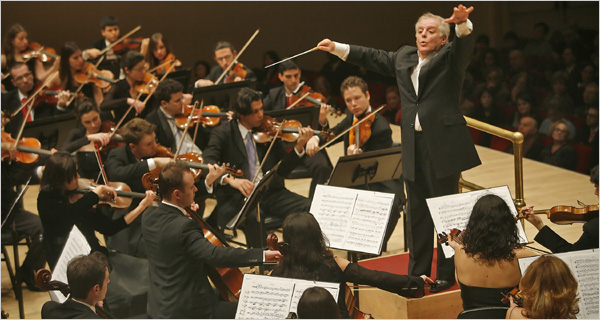
\includegraphics[width=0.9\textwidth]{concert}}
  \end{figure}
  \begin{itemize}[<+->]
  Features come together in an elegant and concise harmony
  \item Reusable Software with native performance!
  \end{itemize}
\end{frame}

\begin{frame}[fragile]{Conclusion: Productivity and Performance}
  \begin{itemize}[<+->]
  \item \emph{Fastest} Compilation of \emph{Fast} Code gives
  \item New level of productivity
  \item And statically Checked gives
  \item New level of correctness an in turn safety
  \item This is a Game-Changer
  \item Flexibility: Fulfils more needs than any other language
  \end{itemize}
\end{frame}

\begin{frame}[fragile]{Final Words}
  \begin{itemize}[<+->]
  \item Computing: Extension of the Intellect
  \item It's human to err so\ldots
  \item Let Compilers help correct us and
  \item Ask not..\\
    what D can do for you but...\\
    what you can do for D!
  \end{itemize}
\end{frame}

\begin{frame}[fragile]{The End}
  \begin{figure}
    \fbox{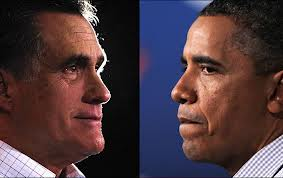
\includegraphics[width=0.8\textwidth]{candidate}}
  \end{figure}
  \emph{Let's} make the best candidate win!
\end{frame}

% %%%%%%%%%%%%%%%%%%%%%%%%%%%%%%%%

\end{document}

%%% Local Variables:
%%% mode: latex
%%% TeX-master: t
%%% End:
